\chapter{Resultados e Discussões}

\section{Resultados para $ F_0 $}
\subsection{Adaptação do filtro}

Os resultados da adaptação do filtro para uma força $F_0(t) = A_0 sin(2\pi f_0 t)$ com $ N=1000 $  e $ SNR = 90 $ são mostrados na \cref{fig:F0_1000_90_conv}. O número de coeficientes do filtro ($ N_c $) e o fator de convergência ($ \mu $) utilizados são apresentados na figura.

\begin{figure}[!h]
	\centering
	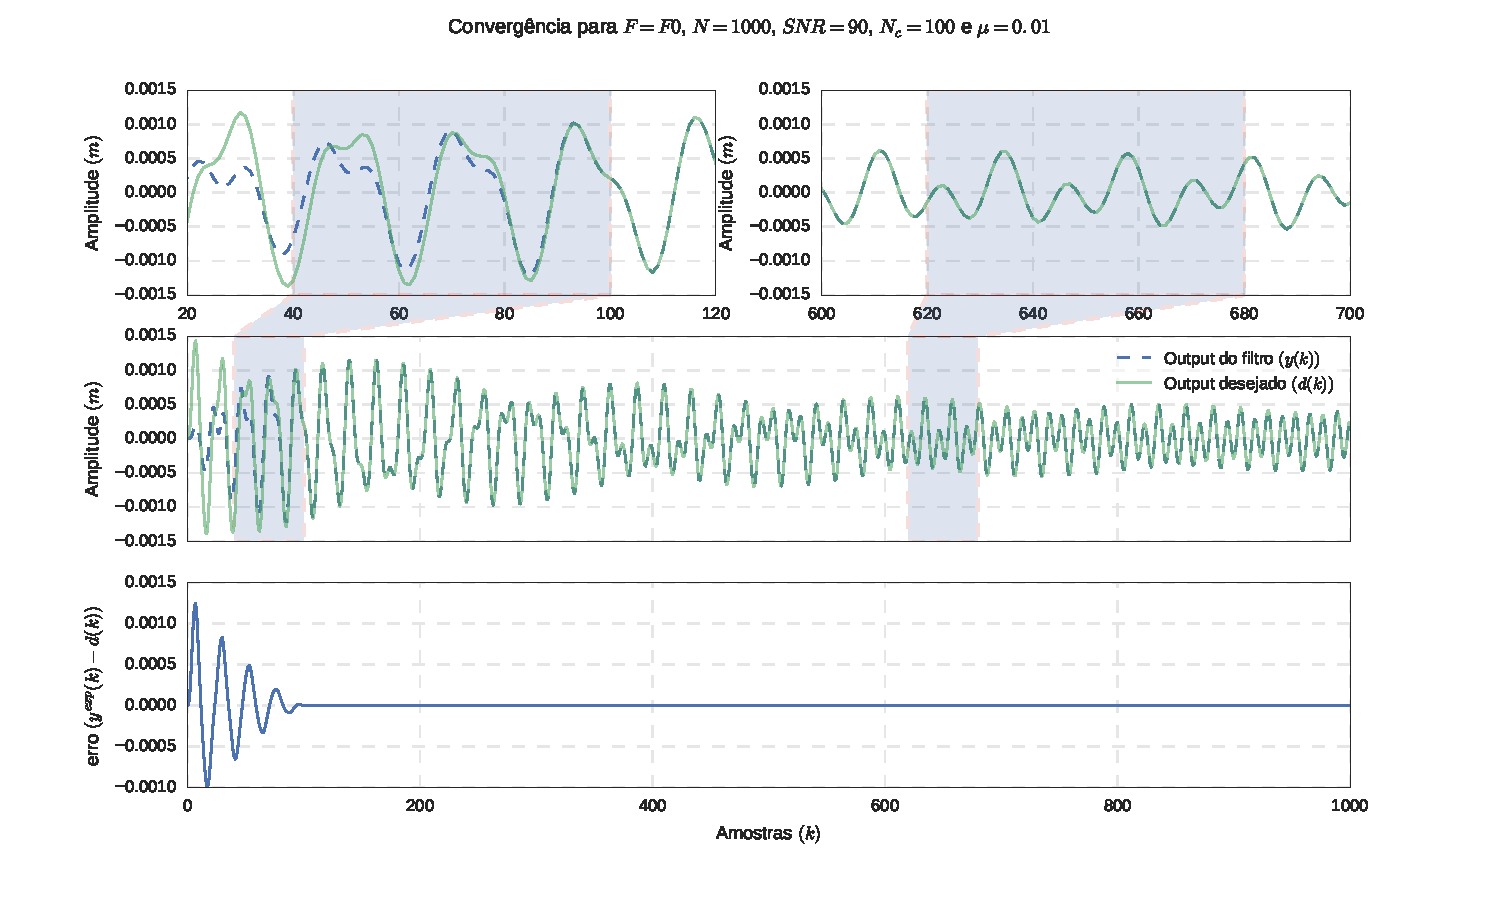
\includegraphics[scale=0.7]{F0_1000_90_conv}
	\caption{Evolução do filtro para $ F=F_0 $, $ N=1000 $ e $ SNR=90 $.}
	\label{fig:F0_1000_90_conv}
\end{figure}

Para o caso do seno puro podemos o filtro tem uma convergência rápida e com menos de 100 iterações o erro já é próximo de zero. 

Na \cref{fig:F0_1000_10_conv} são apresentados os resultados para $ N=1000 $ e $ SNR=10 $. Podemos observar que, mesmo com um nível de ruído mais elevado, o algoritmo apresentou uma convergência rápida.

\begin{figure}
	\centering
	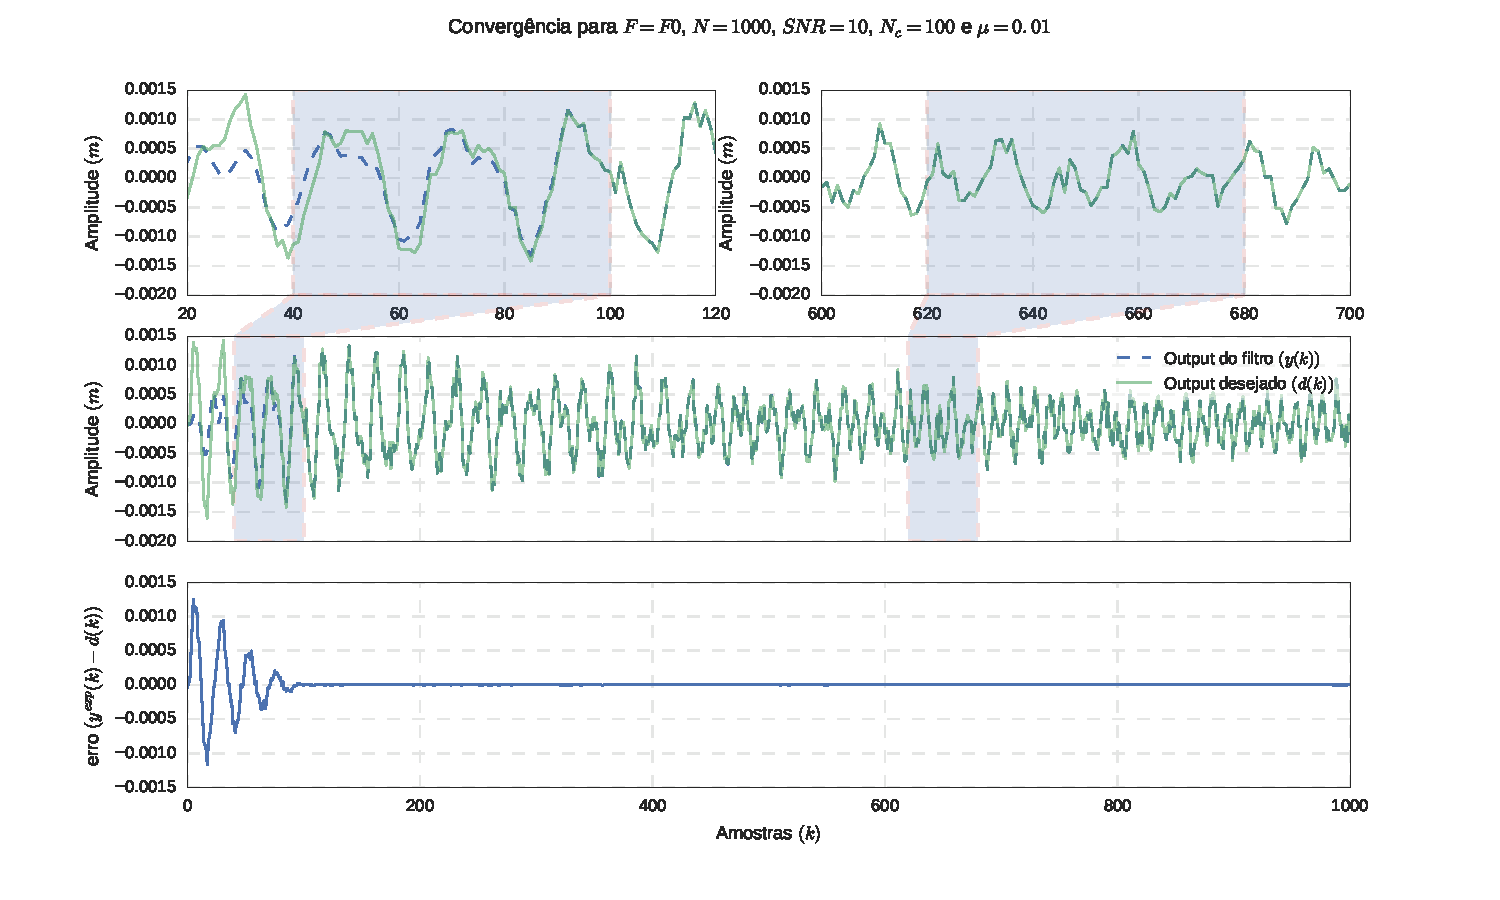
\includegraphics[scale=0.7]{F0_1000_10_conv}
	\caption{Evolução do filtro para $ F=F_0 $, $ N=1000 $ e $ SNR=10 $.}
	\label{fig:F0_1000_10_conv}
\end{figure}

\subsection{FRF do filtro}

Na \cref{fig:F0_1000_90_FRF_med_False} é apresentada a FRF do filtro obtido com $ SNR=90 $ considerando o último vetor de coeficientes, e na \cref{fig:F0_1000_90_FRF_med_True} é apresentada a FRF considerando o vetor obtido através do valor esperado dos coeficientes tomando por base as observações da segunda metade do vetor de dados. A \cref{fig:F0_1000_10_FRF} apresenta os resultados para $ SNR=10 $. 

Podemos observar que FRF do filtro obtido não apresenta bons resultados, aproximando-se do valor esperado apenas na frequência de excitação (\SI{34}{\radian \per \s}). Podemos notar um aumento na amplitude próxima à primeira frequência natural do sistema, mas o valor não se aproxima do esperado. Outro ponto importante é que, para este caso, a FRF do filtro não se mostrou sensível ao nível de ruído. A utilização do último vetor de coeficientes $ w $ ou do valor esperado para a segunda metade do vetor de dados também não teve impacto significativo na resposta. 

\begin{figure}
	\centering
	\begin{subfigure}{0.9\textwidth}
		\centering
		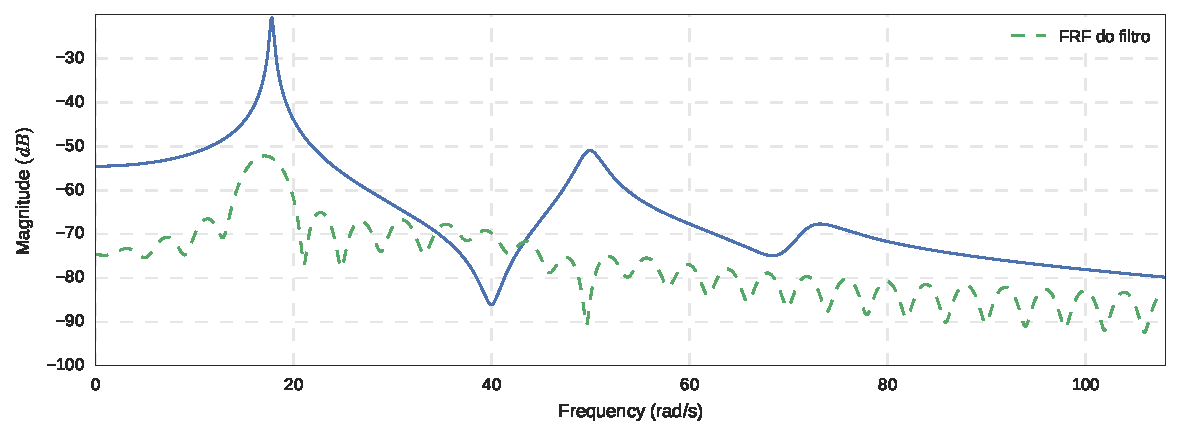
\includegraphics[width=0.9\linewidth]{F0_1000_90_FRF_med_False}
		\caption{último vetor $ w $}
		\label{fig:F0_1000_90_FRF_med_False}
	\end{subfigure}
	\begin{subfigure}{0.9\textwidth}
		\centering
		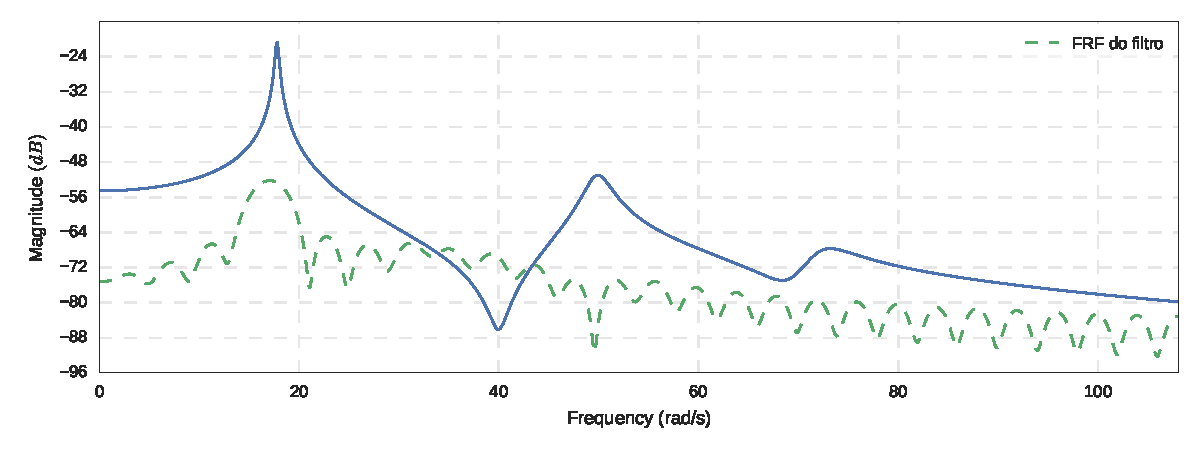
\includegraphics[width=0.9\linewidth]{F0_1000_90_FRF_med_True}
		\caption{valor médio de $ w $}
		\label{fig:F0_1000_90_FRF_med_True}
	\end{subfigure}
	\caption{FRF do filtro obtido para $ F=F_0 $, $ N=1000 $ e $ SNR=90 $.}
\end{figure}

\begin{figure}
	\centering
	\begin{subfigure}{0.9\textwidth}
		\centering
		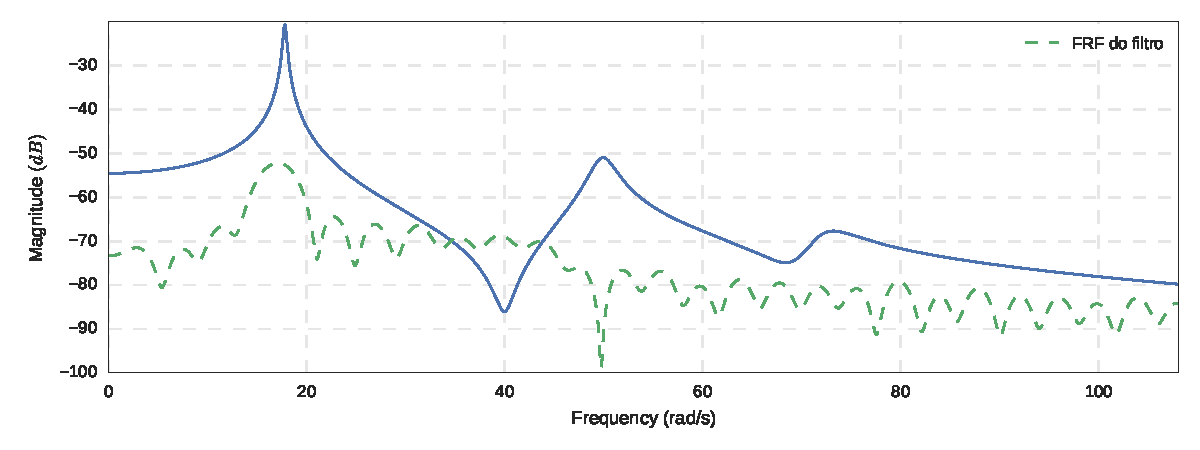
\includegraphics[width=0.9\linewidth]{F0_1000_10_FRF_med_False}
		\caption{último vetor $ w $}
		\label{fig:F0_1000_10_FRF_med_False}
	\end{subfigure}
	\begin{subfigure}{0.9\textwidth}
		\centering
		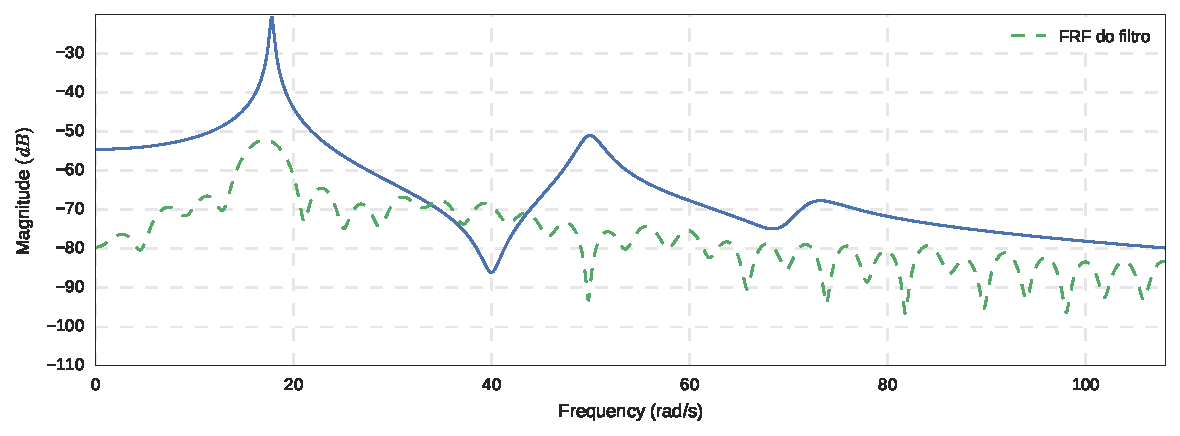
\includegraphics[width=0.9\linewidth]{F0_1000_10_FRF_med_True}
		\caption{valor médio de $ w $}
		\label{fig:F0_1000_10_FRF_med_True}
	\end{subfigure}
	\caption{FRF do filtro obtido para $ F=F_0 $, $ N=1000 $ e $ SNR=10 $.}
	\label{fig:F0_1000_10_FRF}
\end{figure}

\subsection{Predição}

Para analisarmos a predição do filtro, foi escolhida uma força arbitrária $ F_3 $ conforme \cref{eq:F_3}

\begin{equation}\label{eq:F_3}
F_3 = B_1 sin(\omega_1 t)
+ B_2 sin(\omega_2 t)
+ B_3 sin(\omega_3 t)
+ \nu
\end{equation}
onde $ B_1=\SI{1}{\N} $, $ B_2=\SI{2}{\N}$ , $ B_3=\SI{3}{\N} $, $ \omega_1= \SI{14}{\radian \per \s} $, $ \omega_2= \SI{40}{\radian \per \s} $, $ \omega_3= \SI{65}{\radian \per \s} $ e $ \nu $ é um ruído branco de variância 1.

A 

\begin{figure}[h]
	\centering
	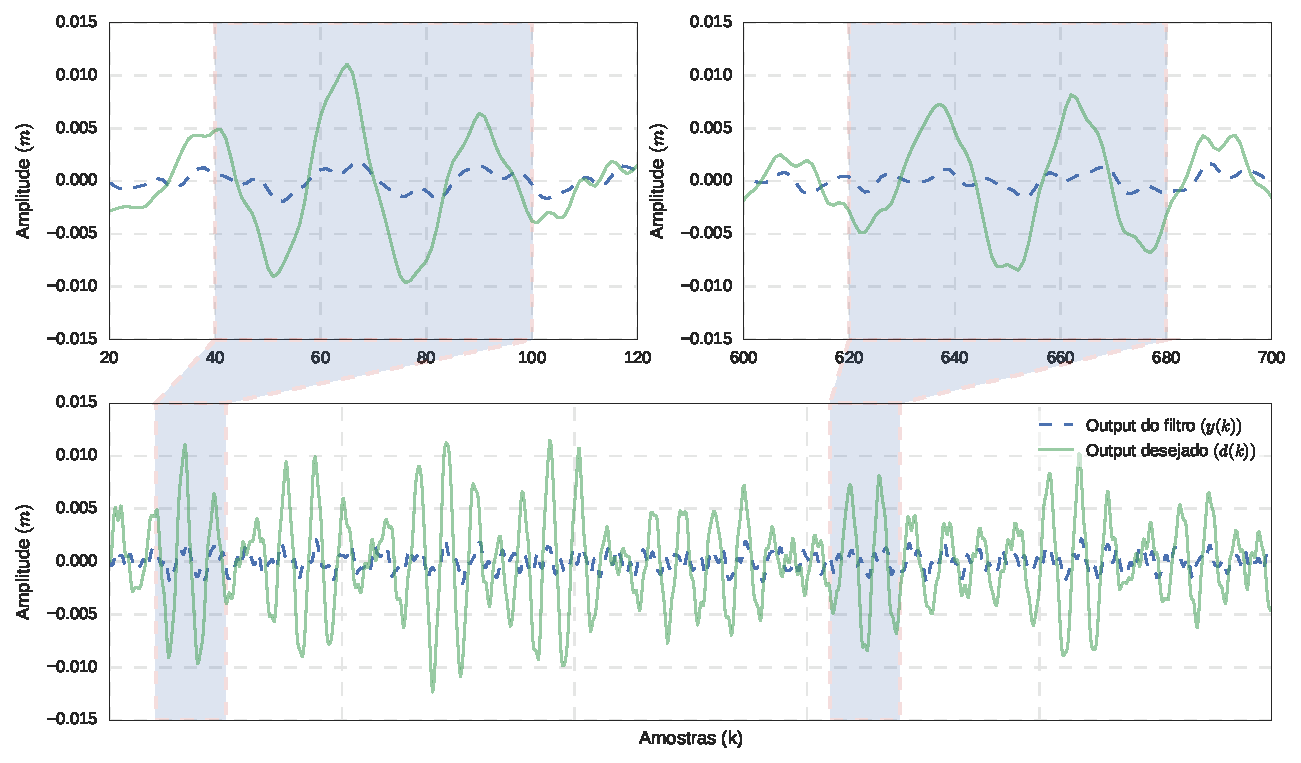
\includegraphics[scale=0.6]{F0_1000_90_pred}
	\caption{Predição do filtro obtido com $ F=F_0 $, $ N=1000 $ e $ SNR=90 $.}
	\label{fig:F0_1000_90_pred}
\end{figure}


Assim como mostrado por \citet{castello2005experimental}, no caso analisado o fenômeno de anti-ressonância também não foi capturado pelo LMS.

